\documentclass[notitlepage, letterpaper, 12pt]{report}
\usepackage[left=1in, right=1in, top=1in, bottom=1in]{geometry}
\usepackage[american]{babel}
\usepackage{graphicx}
\usepackage{titling}
\usepackage{float}
\usepackage{appendix}
\usepackage{mathtools}

\usepackage{listings}
\usepackage{color}

\definecolor{dkgreen}{rgb}{0,0.6,0}
\definecolor{gray}{rgb}{0.5,0.5,0.5}
\definecolor{mauve}{rgb}{0.58,0,0.82}

\lstset{frame=tb,
  language=C++,
  aboveskip=3mm,
  belowskip=3mm,
  showstringspaces=false,
  columns=flexible,
  basicstyle={\small\ttfamily},
  numbers=none,
  numberstyle=\tiny\color{gray},
  keywordstyle=\color{blue},
  commentstyle=\color{dkgreen},
  stringstyle=\color{mauve},
  breaklines=true,
  breakatwhitespace=true,
  tabsize=3
}


\pretitle{\begin{center}\Huge\bfseries}
\posttitle{\par\end{center}\vskip 0.5em}
\preauthor{\begin{center}\Large\ttfamily}
\postauthor{\end{center}}
\predate{\par\large\centering}
\postdate{\par}


\title{Performance Analysis}
\author{Blair Urish and Dan Wagner}
\date{\today}


\begin{document}
\maketitle

\section*{Introduction}
Our task in this homework assignment was to evaluate a hybrid method in which MPI is used to distribute the program across multiple processes and OpenMP
is used to add parallelization on each core.  
The nodes in the Beocat cluster used for this experiment had dual 8-Core Xeon E5-2690s or dual 10-Core Xeon E5-2690 V2s with available RAM ranging from 64GB to 384GB. The nodes were running Linux 4.8.9 and the compiler used was G++ 4.9.4 at 
optimization level 2. For all experiments, between 1 and 16 cores were used.  

\section*{Numerical Integration of Easom's function}

The first task was to write a program that would perform numerical integration on Easom's function:

\[f(x,y) = -\cos(x)*\sin(y)*\exp(-((x - \pi)*(x - \pi) + (y - \pi)*(y - \pi))) \]

The first MPI version worked in a very straightforward way. All processes began by taking in the starting and ending
values for both x and y and immediately beginning their portion of the work. The work was divided up in even partitions when possible.
When all nodes finished computing their portion of the result, an MPI reduction was performed to reduce all local results into one global result.
The rank 0 process would then output this global result and the amount of time taken to compute it. 

Next, we took this initial MPI version and slightly modified it to use OpenMP on each individual node. For this program, there was only
one area that it would make sense to parallelize, and that was the main loop for computing the integral. With OpenMP, the modification to make the
loop run in parallel was only one line. We used the parallel for directive with the option to perform an OpenMP reduction on the variable which keeps
track of the result. This one line broke the loop up into 4 parts for each of the 4 OpenMP threads that we requested. OpenMP automatically handles
race conditions with the result variable due to our use of the reduction directive. 

Below is a chart which compares the runtime of the two versions:

\begin{figure}[H]
	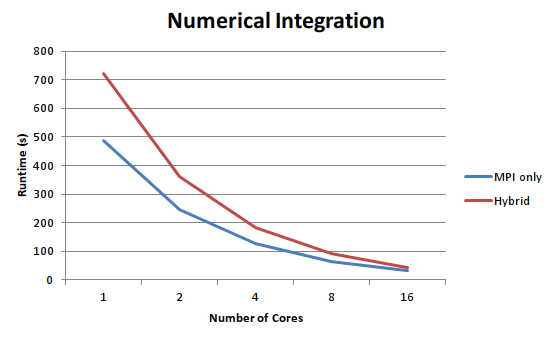
\includegraphics[width=\linewidth,height=8cm,keepaspectratio]{q1.png}
	\caption[Numerical Integration Runtime]{Numerical Integration Runtime}
	\label{fig:arch}
\end{figure}

As one can see, the hybrid MPI/OpenMP version was actually slower than the standalone MPI version. This is likely due to the method in which
MPI was invoked. Generally, each MPI process used 1 core on as many different machines as possible. Attempting to spawn 4 threads on a single core will
not yield a significant performance improvement, especially considering that the cores on Beocat do not have hyperthreading enabled. However, both versions
still had significant performance improvements over the serial implementation. 

Finally, the amount of communication in this program is very minimal. The nodes do not need to communicate until they have finished their computations. At that point,
they will simply send their local result (8 bytes) to the rank 0 node where they will be added together. 

\section*{Monte-Carlo Analysis}
Two programs were written to find the minimum of the given formula:
\[f(x) = \cos(x)+((\lvert7.0-x\rvert^{2.0/15.0}) + 2*(\lvert5.0-x\rvert^{4.0/35.0})) \]
The programs were responsible for taking two points: a starting and ending value for x.  These points were broadcast to every MPI process.  Every process subdivided the range and performed a Monte Carlo analysis to find the value of x that minimized the function.

The MPI implementation was rather simple.  The root node transmitted the starting and ending points to each process, each of which then underwent 1M iterations of Monte Carlo.  The processes found their local minimums and transmitted this information back to the root node.  The root node evaluated each local minimum and found the absolute maximum.  This implementation was simple due to not having to worry about threads and critical sections when updating the local minimum and value of x.  In terms of communication, the root node transmitted two floating point values (4 bytes each) at the start.  Then, each process sent their minimum back (4 bytes).  Overall, message sizes were relatively small.  At the maximum of 16 processes, the number of messages sent were around 45: two floats were broadcast to fifteen other processes, and each of the fifteen other processes sent back their local minimum.  The size of the messages were 4 bytes each, which totaled 180 bytes of data sent.  As the number of processes increased, the run time increased but the results became more accurate (each process was running 1M iterations on a subset of the data).

\begin{figure}[H]
	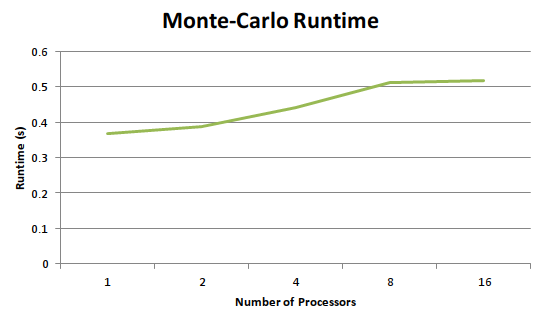
\includegraphics[width=\linewidth,height=8cm,keepaspectratio]{q2.png}
	\caption[Monte Carlo Runtime]{Monte Carlo Runtime}
	\label{fig:arch}
\end{figure}

The hybrid OpenMP \& MPI implementation was not as trivial.  The root node transmitted the start and end points as before, and each process still performed their Monte Carlo iterations.  Race conditions became apparent when finding the minimizing x value.  When each thread needed to compare its local minimum to the overall minimum from the process, a lock was acquired.  The thread changed the value of the overall minimum if needed, and then released the lock.  This technique was detrimental to the performance of the process, as each thread could not execute its iterations without substantial idle time waiting for the lock.  Communication stayed the same, as the threads operated on their processes and only the processes needed to communicate.  OpenMP was successful in reducing the run time of each set, as expected.  As the number of threads increased, the run time of the program generally decreased.  Interestingly, the run time with eight threads per processor was higher than the 2 or 4 threads, but was still lower than one thread.  This is most likely due to more threads contending for the lock to access the minimum values.

\begin{figure}[H]
	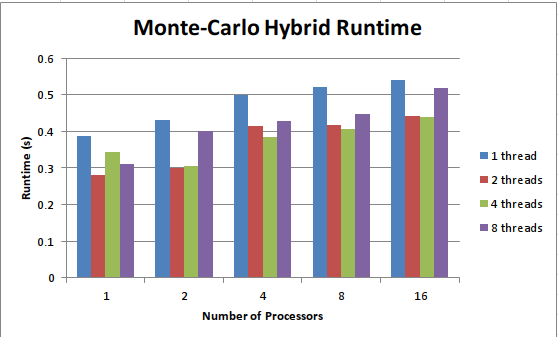
\includegraphics[width=\linewidth,height=8cm,keepaspectratio]{q2-hybrid.png}
	\caption[Monte Carlo Hybrid Runtime]{Monte Carlo Hybrid Runtime}
	\label{fig:arch}
\end{figure}

\section*{Distributed Standard Deviation}

The last application we had to make was a program to calculate the standard deviation of a random set of numbers.
The program was required to have a node act as a server which would actually perform the calculation of the standard deviation, and the
client nodes would generate parts of the sample space and perform some intermediate calculations required by the server. 

For our program, each client was assigned a portion of the sample space to generate and calculate the mean of. Each of the means from the clients are then
transmitted to the server where the mean of the entire sample space will be calculated. This mean is sent back to all of the clients and they will each
calculate the sum of the squares for their sample space using the mean received from the server. 
This is the most expensive part of the application. When this operation is complete, each client will
send their result back to the server where the sums of squares are added together and then the final calculation is performed. 

As for the hybrid version of this application, OpenMP was used to parallelize the calculation of the mean on each client and the calculation of the sums of squares. 
These two operations are the most computationally expensive parts of the program, so it makes sense to parallelize them. Like the numerical integration program, an
OpenMP reduction operation was used to calculate the sums in both of these loops. This addresses the race condition that results from two threads trying to write to the
result variable at the same time.

Below is a chart showing the results when running with a sample space of 1 billion integers:

\begin{figure}[H]
	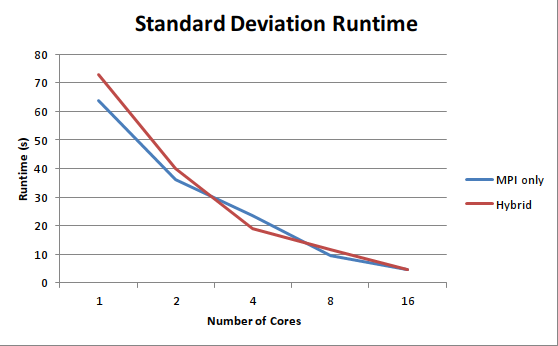
\includegraphics[width=\linewidth,height=8cm,keepaspectratio]{q3.png}
	\caption[Standard Deviation Runtime]{Standard Deviation Runtime}
	\label{fig:arch}
\end{figure}

As with the numerical integration program, the OpenMP version was not significantly faster than the MPI only version. This is for the same reason as before. Since each MPI process
is running on only one core, the program does not see a signficant benefit from adding additional threads.  

The amount of time the nodes spend communicating is minimal assuming the sample space is not very small. Overall, the amount of data transferred will be 64 bytes * number of clients 
and the number of clients will always be 1 minus the number of processors alloted. This is a very small amount of data and a small amount of messages, however, if the sample space
is small enough, one would notice the communication becoming the program's bottleneck instead of the actual calculations. 

\section*{Conclusion}
Overall, the hybrid versions did not perform better than the MPI only versions of the three programs tested. Performance could be improved in the hybrid versions if the MPI settings
were adjusted to allow access to more than 1 core, or if the programs were run on cores with hyperthreading enabled. 

\newpage

\subsection*{Appendix A - q1.cpp}
\begin{lstlisting}
#include <iostream>
#include <cmath>
#include <mpi.h>

#define R_SZ 0.00001

int num_threads = 1;

inline double f(int x, int y)
{
	return -std::cos(x) * std::sin(y) * std::exp(-((x - M_PI)*(x - M_PI) + (y - M_PI)*(y - M_PI)));	
}

double do_work(int rank, int x_start, int x_end, int y_start, int y_end)
{
	int iters = x_end - x_start;
	int loop_start = (rank * (iters / num_threads));
	int loop_end = loop_start + (iters / num_threads);
	loop_start += x_start;
	loop_end += x_start;

	if (rank == num_threads-1) loop_end = x_end;

	std::cout << "rank: " << rank << " start: " << loop_start << " end: " << loop_end << std::endl;	

	double result = 0.0;
	for (int i = loop_start; i < loop_end; ++i)
	{
		for (int j = y_start; j < y_end; ++j)
		{
			result += R_SZ*R_SZ*f(x_start+i*R_SZ, y_start+j*R_SZ);	
		}
	}

	return result;
}

double myclock() 
{
	static time_t t_start = 0;  // Save and subtract off each time

	struct timespec ts;
	clock_gettime(CLOCK_REALTIME, &ts);
	if( t_start == 0 ) t_start = ts.tv_sec;

	return (double) (ts.tv_sec - t_start) + ts.tv_nsec * 1.0e-9;
}

int main(int argc, char** argv)
{
	if (argc != 5)
	{
		std::cout << "usage: " << argv[0] << " [x_start] [x_end] [y_start] [y_end]" << std::endl;
		return 1;
	}

	int x_start = std::atoi(argv[1]);
	int x_end = std::atoi(argv[2]);
	int y_start = std::atoi(argv[3]);
	int y_end = std::atoi(argv[4]);
    int rc;
	int rank = 0;
	double tstart, ttotal;

    if ((rc = MPI_Init(&argc, &argv)) != MPI_SUCCESS)
   	{
		std::cout << "error: cannot start mpi" << std::endl;
		MPI_Abort(MPI_COMM_WORLD, rc);	  
    } 

	
	MPI_Comm_size(MPI_COMM_WORLD,&num_threads);
	MPI_Comm_rank(MPI_COMM_WORLD,&rank);

	tstart = myclock();	
	tstart = myclock();	

	double result = do_work(rank, x_start, x_end, y_start, y_end);

	double global_result;
	MPI_Reduce(&result, &global_result, 1, MPI_DOUBLE, MPI_SUM, 0, MPI_COMM_WORLD);

   	ttotal = myclock() - tstart;

	if (rank == 0)
	{
		std::cout << "Result: " << global_result << std::endl;
		std::cout << "Time: " << ttotal << " seconds" << std::endl;
	}

	MPI_Finalize();
	return 0;
}
\end{lstlisting}
\newpage

\subsection*{Appendix B - q1-hybrid.cpp}
\begin{lstlisting}
#include <iostream>
#include <cmath>
#include <mpi.h>
#include <omp.h>

#define R_SZ 0.00001
#define NUM_OMP_THREADS 4

int num_threads = 1;

inline double f(int x, int y)
{
	return -std::cos(x) * std::sin(y) * std::exp(-((x - M_PI)*(x - M_PI) + (y - M_PI)*(y - M_PI)));	
}

double do_work(int rank, int x_start, int x_end, int y_start, int y_end)
{
	int iters = x_end - x_start;
	int loop_start = (rank * (iters / num_threads));
	int loop_end = loop_start + (iters / num_threads);
	loop_start += x_start;
	loop_end += x_start;

	if (rank == num_threads-1) loop_end = x_end;

	std::cout << "rank: " << rank << " start: " << loop_start << " end: " << loop_end << std::endl;	

	double result = 0.0;
	int i,j;
#pragma omp parallel for private(i,j) reduction(+: result)
	for (i = loop_start; i < loop_end; ++i)
	{
		for (j = y_start; j < y_end; ++j)
		{
			result += R_SZ*R_SZ*f(x_start+i*R_SZ, y_start+j*R_SZ);	
		}
	}

	return result;
}

double myclock() 
{
	static time_t t_start = 0;  // Save and subtract off each time

	struct timespec ts;
	clock_gettime(CLOCK_REALTIME, &ts);
	if( t_start == 0 ) t_start = ts.tv_sec;

	return (double) (ts.tv_sec - t_start) + ts.tv_nsec * 1.0e-9;
}

int main(int argc, char** argv)
{
	if (argc != 5)
	{
		std::cout << "usage: " << argv[0] << " [x_start] [x_end] [y_start] [y_end]" << std::endl;
		return 1;
	}

	int x_start = std::atoi(argv[1]);
	int x_end = std::atoi(argv[2]);
	int y_start = std::atoi(argv[3]);
	int y_end = std::atoi(argv[4]);
    int rc;
	int rank = 0;
	double tstart, ttotal;

    if ((rc = MPI_Init(&argc, &argv)) != MPI_SUCCESS)
   	{
		std::cout << "error: cannot start mpi" << std::endl;
		MPI_Abort(MPI_COMM_WORLD, rc);	  
    } 

	
	MPI_Comm_size(MPI_COMM_WORLD,&num_threads);
	MPI_Comm_rank(MPI_COMM_WORLD,&rank);
	omp_set_num_threads(NUM_OMP_THREADS);

	tstart = myclock();	
	tstart = myclock();	

	double result = do_work(rank, x_start, x_end, y_start, y_end);

	double global_result;
	MPI_Reduce(&result, &global_result, 1, MPI_DOUBLE, MPI_SUM, 0, MPI_COMM_WORLD);

   	ttotal = myclock() - tstart;

	if (rank == 0)
	{
		std::cout << "Result: " << global_result << std::endl;
		std::cout << "Time: " << ttotal << " seconds" << std::endl;
	}

	MPI_Finalize();
	return 0;
}
\end{lstlisting}
\newpage

\subsection*{Appendix C - q2.cpp}
\begin{lstlisting}
#include <stdlib.h>
#include <cstdlib>
#include <stdio.h>
#include <string.h>
#include <iostream>
#include <float.h>
#include <cmath>
#include <mpi.h>

// Number of iterations in Monte Carlo
#define NUM_ITER 1000000

// Floats for single precision decimal values
float end_x, start_x, min_x;

// Number of MPI processes and OMP threads
int nprocs, nthreads;
float *minimum;
float local_min;
void *eval_func(void*);
double myclock(void);
float f(float);

// Function to minimize.
float f(float x) {
	return cos(x) + (pow(fabs(7.0 - x), 2.0/15.0)) + 2*(pow(fabs(5.0 - x), 4.0/35.0));
}

// Evaluate the function at points using Monte Carlo analysis.
void *eval_func(void* rank) {
	// Segment the range based on rank.
	int ID = *((int *) rank);
	float start = (ID * ((end_x - start_x) / nprocs)) + start_x; 
	float end = start + ((end_x - start_x) / nprocs); 
	local_min = FLT_MAX;
	float f_min = FLT_MAX;
	float random, min;
	printf("Rank %d going from %f to %f\n", ID, start, end);
	// Generate a random floating point number in the subdivided range.
	for (int x = 0; x < NUM_ITER; x++) {
		random = (rand() * (end - start) / RAND_MAX) + start;
		min = f(random);
		if (min < f_min) {
			f_min = min;
			local_min = random;
		}
	}
	printf("local min from rank %d: %f\n", ID, local_min);
	// Send the value that minimizes the function back to the main process.
	if (ID != 0) {
		printf("Rank %d sending local_min %f\n", ID, local_min);
		MPI_Send(&local_min, 1, MPI_FLOAT, 0, 0, MPI_COMM_WORLD);
	}
	else { printf("Rank 0 storing local_min %f\n", local_min); minimum[0] = local_min; }
}

// Used to compute the amount of time the program takes to run.
double myclock() {
   static time_t t_start = 0;  // Save and subtract off each time

   struct timespec ts;
   clock_gettime(CLOCK_REALTIME, &ts);
   if( t_start == 0 ) t_start = ts.tv_sec;

   return (double) (ts.tv_sec - t_start) + ts.tv_nsec * 1.0e-9;
}

int main(int argc, char *argv[]) {
	int rank;
	double tstart, ttotal;
	nprocs = atoi(getenv("NSLOTS"));

	// Data validation.
	if (argc < 3) {
		std::cout << "Please enter the start and end points." << std::endl;
		return -1;
	}

	// Initialize the MPI processes.
	int rc = MPI_Init(&argc, &argv);
	if (rc != MPI_SUCCESS) {
		std::cout << "Error with MPI." << std::endl;
		MPI_Abort(MPI_COMM_WORLD, rc);
	}
	MPI_Comm_size(MPI_COMM_WORLD, &nprocs);
	MPI_Comm_rank(MPI_COMM_WORLD, &rank);
		
	nthreads = atoi(argv[3]);	
	if (rank == 0) {
		minimum = new float[nprocs];
		// Grab the starting and ending values of x.	
		start_x = atof(argv[1]);
		end_x = atof(argv[2]);
		std::cout << "start, end: " << start_x << ", " << end_x << std::endl;
		tstart = myclock(); tstart = myclock();
	}


	// Broadcast the starting and ending points to processes.
	MPI_Bcast(&start_x, 1, MPI_FLOAT, 0, MPI_COMM_WORLD);
	MPI_Bcast(&end_x, 1, MPI_FLOAT, 0, MPI_COMM_WORLD);
	
	// Evaulate the function to find minimum values.
	eval_func(&rank);

	if (rank == 0) {
		float min = 0;
		MPI_Status stat;
		// Pass back the values to prevent idle processes. 
		for (int i = 1; i < nprocs; i++) {
			MPI_Recv(&min, 1, MPI_FLOAT, i, 0, MPI_COMM_WORLD, &stat);
			printf("Received min %f from rank %d\n", min, i);
			minimum[i] = min; 
		}
		
		min = FLT_MAX;
		min_x = FLT_MAX;
		printf("local_min: %f\n", minimum[0]);
		// Find the global minimum.
		for (int i = 0; i < nprocs; i++) {
			float x = minimum[i];
			float y = f(x);
			printf("x, y: %f, %f\n", x, y);
			if (y < min) { min = y; min_x = x;}	
		}
		ttotal = myclock() - tstart;
		printf("DATA, %f, %d, %d, %lf\n", min_x, nprocs, nthreads, ttotal);	
	}

	// Free memory and clean up. 
	if (rank == 0) delete[] minimum;
	MPI_Finalize();
	return 0;
}

\end{lstlisting}

\newpage

\subsection*{Appendix D - q2-hybrid.cpp}
\begin{lstlisting}
#include <stdlib.h>
#include <cstdlib>
#include <stdio.h>
#include <string.h>
#include <iostream>
#include <float.h>
#include <cmath>
#include <mpi.h>
#include <omp.h>

// Number of iterations in Monte Carlo
#define NUM_ITER 1000000

// Floats for single precision decimal values
float end_x, start_x, min_x;

// Number of MPI processes and OMP threads
int nprocs, nthreads;
float *minimum;
float local_min;
void *eval_func(void*);
double myclock(void);
float f(float);

// Function to minimize via Monte Carlo.
float f(float x) {
	return cos(x) + (pow(fabs(7.0 - x), 2.0/15.0)) + 2*(pow(fabs(5.0 - x), 4.0/35.0));
}

// Evaluate the function at points using Monte Carlo analysis.
void *eval_func(void* rank) {
	// Segment the range based on rank.
	int ID = *((int *) rank);
	float start = (ID * ((end_x - start_x) / nprocs)) + start_x; 
	float end = start + ((end_x - start_x) / nprocs); 
	local_min = FLT_MAX;
	float f_min = FLT_MAX;
	float random, min;
	int x;

	omp_set_dynamic(0);
	omp_set_num_threads(nthreads);
	#pragma omp parallel for shared(f_min, local_min) private(x, min, random)
	// Generate a random floating point number in the subdivided range.
	for (x = 0; x < NUM_ITER; x++) {
		random = (rand() * (end - start) / RAND_MAX) + start;
		min = f(random);
		#pragma omp critical // Getting wrong values 2+ threads
		{
			if (min < f_min) {
				f_min = min;
				local_min = random;
			}
		}
	}

	// Send the value that minimizes the function back to the main process.
	if (ID != 0) MPI_Send(&local_min, 1, MPI_FLOAT, 0, 0, MPI_COMM_WORLD);
	else minimum[0] = local_min;
}

// Used to compute the amount of time the program takes to run.
double myclock() {
   static time_t t_start = 0;  // Save and subtract off each time

   struct timespec ts;
   clock_gettime(CLOCK_REALTIME, &ts);
   if( t_start == 0 ) t_start = ts.tv_sec;

   return (double) (ts.tv_sec - t_start) + ts.tv_nsec * 1.0e-9;
}

int main(int argc, char *argv[]) {
	int rank;
	double tstart, ttotal;
	nprocs = atoi(getenv("NSLOTS"));

	// Data validation.
	if (argc < 3) {
		std::cout << "Please enter the start and end points." << std::endl;
		return -1;
	}
	
	// Initialize the MPI processes.
	int rc = MPI_Init(&argc, &argv);
	if (rc != MPI_SUCCESS) {
		std::cout << "Error with MPI." << std::endl;
		MPI_Abort(MPI_COMM_WORLD, rc);
	}
	MPI_Comm_size(MPI_COMM_WORLD, &nprocs);
	MPI_Comm_rank(MPI_COMM_WORLD, &rank);
		
	if (rank == 0) {
		minimum = new float[nprocs];
		// Grab the starting and ending values of x.
		start_x = atof(argv[1]);
		end_x = atof(argv[2]);
		std::cout << "start, end: " << start_x << ", " << end_x << std::endl;
		tstart = myclock(); tstart = myclock();
	}

	// Grab the number of threads per process from the command line.
	nthreads = atoi(argv[3]);

	// Broadcast the starting and ending points to processes.
	MPI_Bcast(&start_x, 1, MPI_FLOAT, 0, MPI_COMM_WORLD);
	MPI_Bcast(&end_x, 1, MPI_FLOAT, 0, MPI_COMM_WORLD);
	
	// Evaulate the function to find minimum values.
	eval_func(&rank);

	if (rank == 0) {
		float min = 0;
		MPI_Status stat;
		// Pass back the values to prevent idle processes. 
		for (int i = 1; i < nprocs; i++) {
			MPI_Recv(&min, 1, MPI_FLOAT, i, 0, MPI_COMM_WORLD, &stat);
			minimum[i] = min; 
		}
		
		min = FLT_MAX;
		min_x = FLT_MAX;
		// Find the global minimum.
		for (int i = 0; i < nprocs; i++) {
			float x = minimum[i];
			float y = f(x); 
			if (y < min) { min = y; min_x = x;}	
		}
		ttotal = myclock() - tstart;
		printf("DATA, %f, %d, %d, %lf\n", min_x, nprocs, nthreads, ttotal);	
	}

	// Free memory and clean up.
	if (rank == 0) delete[] minimum;
	MPI_Finalize();
	return 0;
}

\end{lstlisting}
\newpage

\subsection*{Appendix E - q3.cpp}
\begin{lstlisting}
#include <iostream>
#include <random>
#include <vector>
#include <cmath>
#include <mpi.h>

#define R_MIN 0
#define R_MAX 1000
#define N 1000000000

int num_threads = 1;

// Generates sample space and returns mean
std::pair<std::vector<int>, int64_t> generate_sample_space(int rank)
{
	int n_per_proc = N / num_threads;

	if (rank == num_threads-1) n_per_proc += N - (n_per_proc*(num_threads-1));

	std::random_device rd;
	std::mt19937 mt(rd());
	std::uniform_int_distribution<int> dist(R_MIN, R_MAX);

	// Generate sample space.
	std::vector<int> sample_space;
	for (int i = 0; i < n_per_proc; ++i)
	{
		auto r = dist(mt);
		sample_space.push_back(r);
	}	

	auto mean = std::accumulate(sample_space.begin(), sample_space.end(), 0LL) / sample_space.size();
	return {sample_space, mean};
}

int64_t find_sum_squares(std::pair<std::vector<int>, int64_t> sample_space_pair)
{
	int64_t sum_squares = 0;
	auto sample_space = sample_space_pair.first;
	auto mean = sample_space_pair.second;
	auto n_per_proc = sample_space.size();
	for (int i = 0; i < n_per_proc; ++i)
	{
		sum_squares += (sample_space[i] - mean)*(sample_space[i] - mean);
	}
	return sum_squares;
}

void do_work(int rank)
{
	auto sample_space_pair = generate_sample_space(rank);
	auto sample_space = sample_space_pair.first;
	auto mean = sample_space_pair.second;

	// send mean back to server so it can be incorporated with other nodes' results.
	MPI_Send(&mean, 1, MPI_INT, 0, 0, MPI_COMM_WORLD);

	// receive new mean from server.
	MPI_Recv(&mean, 1, MPI_INT, 0, 0, MPI_COMM_WORLD, MPI_STATUS_IGNORE);

	auto sum_squares = find_sum_squares({sample_space, mean});

	MPI_Send(&sum_squares, 1, MPI_LONG_LONG, 0, 0, MPI_COMM_WORLD);
}

double myclock() {
   static time_t t_start = 0;  // Save and subtract off each time

   struct timespec ts;
   clock_gettime(CLOCK_REALTIME, &ts);
   if( t_start == 0 ) t_start = ts.tv_sec;

   return (double) (ts.tv_sec - t_start) + ts.tv_nsec * 1.0e-9;
}

int main(int argc, char** argv)
{
    int rc;
	int rank;
	double tstart, ttotal;
    if ((rc = MPI_Init(&argc, &argv)) != MPI_SUCCESS)
   	{
		std::cout << "error: cannot start mpi" << std::endl;
		MPI_Abort(MPI_COMM_WORLD, rc);	  
    } 

	MPI_Comm_size(MPI_COMM_WORLD,&num_threads);
	MPI_Comm_rank(MPI_COMM_WORLD,&rank);

	if (rank == 0)
	{
		tstart = myclock();	
		tstart = myclock();	
		
		int64_t sum_squares = 0;
		if (num_threads > 1)
		{
			std::vector<int> means;
			for (int i = 1; i < num_threads; ++i)
			{
				int mean;
				MPI_Recv(&mean, 1, MPI_INT, i, 0, MPI_COMM_WORLD, MPI_STATUS_IGNORE);
				means.push_back(mean);
			}

			auto new_mean = std::accumulate(means.begin(), means.end(), 0LL) / means.size();

			for (int i = 1; i < num_threads; ++i)
			{
				MPI_Send(&new_mean, 1, MPI_INT, i, 0, MPI_COMM_WORLD);
			}

			for (int i = 1; i < num_threads; ++i)
			{
				int64_t result;
				MPI_Recv(&result, 1, MPI_LONG_LONG, i, 0, MPI_COMM_WORLD, MPI_STATUS_IGNORE);
				sum_squares += result;	
			}
		}
		else
		{
			// single threaded...
			sum_squares = find_sum_squares(generate_sample_space(rank));
		}


		// Compute standard deviation.
		auto sd = std::sqrt(sum_squares / (N-1));
   		ttotal = myclock() - tstart;
		std::cout << "Standard deviation: " << sd << std::endl;
		std::cout << "Time: " << ttotal << " seconds" << std::endl;
		std::cout << "Cores: " << num_threads << std::endl;
	}
	else
	{
		do_work(rank);
	}

	MPI_Finalize();
	return 0;
}
\end{lstlisting}
\newpage

\subsection*{Appendix F - q3-hybrid.cpp}
\begin{lstlisting}
#include <iostream>
#include <random>
#include <vector>
#include <cmath>
#include <mpi.h>
#include <omp.h>

#define R_MIN 0
#define R_MAX 1000
#define N 1000000000
#define NUM_OMP_THREADS 4

int num_threads = 1;

// Generates sample space and returns mean
std::pair<std::vector<int>, int64_t> generate_sample_space(int rank)
{
	int n_per_proc = N / num_threads;

	if (rank == num_threads-1) n_per_proc += N - (n_per_proc*(num_threads-1));

	std::random_device rd;
	std::mt19937 mt(rd());
	std::uniform_int_distribution<int> dist(R_MIN, R_MAX);

	// Generate sample space.
	std::vector<int> sample_space;
	for (int i = 0; i < n_per_proc; ++i)
	{
		auto r = dist(mt);
		sample_space.push_back(r);
	}	

	int64_t sum = 0;
	int i;
#pragma omp parallel for private(i) reduction(+: sum)
	for (i = 0; i < n_per_proc; ++i)
	{
		sum += sample_space[i];
	}	
	auto mean = sum / sample_space.size();

	return {sample_space, mean};
}

int64_t find_sum_squares(std::pair<std::vector<int>, int64_t> sample_space_pair)
{
	int64_t sum_squares = 0;
	auto sample_space = sample_space_pair.first;
	auto mean = sample_space_pair.second;
	auto n_per_proc = sample_space.size();
	
	int i;
#pragma omp parallel for private(i) reduction(+: sum_squares)
	for (i = 0; i < n_per_proc; ++i)
	{
		sum_squares += (sample_space[i] - mean)*(sample_space[i] - mean);
	}

	return sum_squares;
}
void do_work(int rank)
{
	auto sample_space_pair = generate_sample_space(rank);
	auto sample_space = sample_space_pair.first;
	auto mean = sample_space_pair.second;

	// send mean back to server so it can be incorporated with other nodes' results.
	MPI_Send(&mean, 1, MPI_INT, 0, 0, MPI_COMM_WORLD);

	// receive new mean from server.
	MPI_Recv(&mean, 1, MPI_INT, 0, 0, MPI_COMM_WORLD, MPI_STATUS_IGNORE);

	auto sum_squares = find_sum_squares({sample_space, mean});

	MPI_Send(&sum_squares, 1, MPI_LONG_LONG, 0, 0, MPI_COMM_WORLD);
}

double myclock() {
   static time_t t_start = 0;  // Save and subtract off each time

   struct timespec ts;
   clock_gettime(CLOCK_REALTIME, &ts);
   if( t_start == 0 ) t_start = ts.tv_sec;

   return (double) (ts.tv_sec - t_start) + ts.tv_nsec * 1.0e-9;
}

int main(int argc, char** argv)
{
    int rc;
	int rank;
	double tstart, ttotal;
    if ((rc = MPI_Init(&argc, &argv)) != MPI_SUCCESS)
   	{
		std::cout << "error: cannot start mpi" << std::endl;
		MPI_Abort(MPI_COMM_WORLD, rc);	  
    } 

	MPI_Comm_size(MPI_COMM_WORLD,&num_threads);
	omp_set_num_threads(NUM_OMP_THREADS);
	MPI_Comm_rank(MPI_COMM_WORLD,&rank);
	
	if (rank == 0)
	{
		tstart = myclock();	
		tstart = myclock();	

		int64_t sum_squares = 0;

		if (num_threads > 1)
		{
			std::vector<int> means;
			for (int i = 1; i < num_threads; ++i)
			{
				int mean;
				MPI_Recv(&mean, 1, MPI_INT, i, 0, MPI_COMM_WORLD, MPI_STATUS_IGNORE);
				means.push_back(mean);
			}

			auto new_mean = std::accumulate(means.begin(), means.end(), 0LL) / means.size();

			for (int i = 1; i < num_threads; ++i)
			{
				MPI_Send(&new_mean, 1, MPI_INT, i, 0, MPI_COMM_WORLD);
			}

			for (int i = 1; i < num_threads; ++i)
			{
				int64_t result;
				MPI_Recv(&result, 1, MPI_LONG_LONG, i, 0, MPI_COMM_WORLD, MPI_STATUS_IGNORE);
				sum_squares += result;	
			}
		}
		else
		{
			sum_squares = find_sum_squares(generate_sample_space(rank));
		}
		// Compute standard deviation.
		auto sd = std::sqrt(sum_squares / (N-1));
   		ttotal = myclock() - tstart;
		std::cout << "Standard deviation: " << sd << std::endl;
		std::cout << "Time: " << ttotal << " seconds" << std::endl;
	}
	else
	{
		do_work(rank);
	}

	MPI_Finalize();
	return 0;
}
\end{lstlisting}
\end{document}
